%Modified from a template provided by Jennifer Pan, August 2011

\documentclass[10pt,letter]{article}
	% basic article document class
	% use percent signs to make comments to yourself -- they will not show up.
\usepackage{pdfsync}
\usepackage{amsmath}
\usepackage{amssymb}
\usepackage{amsthm}
\usepackage[makeroom]{cancel}
	% packages that allow mathematical formatting

\usepackage{graphicx}
	% package that allows you to include graphics
\graphicspath{ {./images/} }


\usepackage{subcaption}

\usepackage{setspace}
	% package that allows you to change spacing

\onehalfspacing
	% text become 1.5 spaced

\usepackage{fullpage}
% package that specifies normal margins

\usepackage[parfill]{parskip}

\newtheorem*{thm}{Theorem}
\newtheorem{nthm}{Theorem}
\newtheorem{lem}{Lemma}

\begin{document}
	% line of code telling latex that your document is beginning

\title{Problem Set 4}

\author{Katherine Cheng, Richard Davis, Marty Keil}

% \date{Friday April 10, 2015}
	% Note: when you omit this command, the current date is automatically included
 
\maketitle 
	% tells latex to follow your header (e.g., title, author) commands.

\section*{Problem One: Properties of Functions}

\begin{enumerate}
\item[1.] Injection
\item[2.] Function
\item[3.] Injection
\item[4.] Function
\item[5.] Non-function
\item[6.] Injection
\item[7.] Non-function
\item[8.] Non-function
\item[9.] Non-function
\item[10.] Bijection
\item[11.] Injection
\item[12.] Surjection
\item[13.] Bijection
\end{enumerate}

\section*{Problem Two: Cartesian Products and Cardinalities}

\paragraph{i.} Using the function $f: A \times B \rightarrow C \times D$ defined as $f(a, b) = (g(a), h(b))$, prove that if $A$, $B$, $C$, and $D$ are sets where $|A| = |C|$ and $|B| = |D|$, then we have $|A \times C| = |C \times D|$. Specifically, prove that $f$ is a bjiection between $A \times B$ and $C \times D$. 

\begin{thm} If $A$, $B$, $C$, and $D$ are sets where $|A| = |C|$ and $|B| = |D|$, then we have $|A \times B| = |C \times D|$. 
\end{thm}

\begin{proof} Because $|A| = |C|$, we know from the definition of equal cardinalities that there is a bijection $g: A \rightarrow C$. Likewise, because $|B| = |D|$ we know there is a bijection $h: B \rightarrow D$. In the definition of the function $f(a, b)$, the ordered-pair output is determined by $(g(a), h(b))$. Let $g(a)$ and $h(b)$ both be the bijections that map every member of $A$ to $C$ and every member of $B$ to $D$. 

If $f(a, b)$ is an injection, this means that $\forall (a_1, b_1) \in A \times B .\ \forall (a_2, b_2) \in A \times B .\ f(a_1, b_1) = f(a_2, b_2) \rightarrow (a_1, b_1) = (a_2, b_2)$. Because $f(a_1, b_1) = (g(a_1), h(b_1))$ and $f(a_2, b_2) = (g(a_2), h(b_2))$, this means that $(g(a_1), h(b_1)) = (g(a_2), h(b_2))$ and furthermore that $g(a_1) = g(a_2)$ and $h(b_1) = h(b_2)$. Because $g(x)$ and $h(x)$ are bijections, we know that $a_1 = a_2$ and $b_1 = b_2$. This proves that $f(a, b)$ is an injection.

If $f(a, b)$ is a surjection, this means that $\forall (c, d) \in C \times D .\ \exists (a, b) \in A \times B .\ f(a, b) = (c, d)$. Because $f(a, b) = (g(a), h(b))$, and because $g(a)$ and $h(b)$ are bijections, we know that for any choice of $c$ we can find some $a$ such that $g(a) = c$ and for any choice of $d$ we can find some $b$ such that $h(b) = d$. This means that for any ordered pair $(c, d)$ we can find some $a$ and some $b$ such that $(c, d) = (g(a), h(b))$. This proves that $f(a, b)$ is a surjection. 

Because $f(a, b)$ is both an injection and a surjection, this proves that $f(a, b)$ is a bijection.

\end{proof}

\paragraph{ii.} Prove that $|\mathbb{N}^k| = |\mathbb{N}|$ for all nonzero $k \in \mathbb{N}$. This result means that for any nonzero finite $k$, there are the same number of $k$-tuples of natural numbers as natural numbers.

\begin{thm} For all nonzero $k \in \mathbb{N}$, $|\mathbb{N}^k| = |\mathbb{N}|$. 
\end{thm}

\begin{proof} By induction. We can define the Cartesian power of a set as follows. For any set $A$ and any natural number $n$, we define $A^n$ inductively:
\begin{align*}
A^1 &= A \\
A^{n+1} &= A \times A^n (\text{for } n \ge 1)\\
\end{align*}
Let $P(n)$ be the statement that ``for all nonzero $n \in \mathbb{N}$, $|\mathbb{N}^n| = |\mathbb{N}|$.'' For our base case we have $P(1)$, that $|\mathbb{N}| = |\mathbb{N}|$. This is a tautology and true.

For our inductive hypothesis, assume that $P(k)$ holds for some nonzero $k$. We will show that $P(k+1)$ is also true. $P(k+1)$ means that $|\mathbb{N}^{k+1}| = |\mathbb{N} \times \mathbb{N}^k|$. From our inductive hypothesis we know that $|\mathbb{N}^k| = |\mathbb{N}|$. From our previous result we know that this allows us to rewrite $|\mathbb{N} \times \mathbb{N}^k|$ as $|\mathbb{N} \times \mathbb{N}|$. This can also be written as $|\mathbb{N}^2|$. From lecture we know that $|\mathbb{N}| = |\mathbb{N}^2|$. Putting this all together we prove that $P(k+1)$ is true.
\end{proof}


\section*{Problem Three: Understanding Diagonalization: Richard}

\paragraph{i.} The diagonal set for this choice is \mathbb{N}. No member of the natural numbers can ever map to this set because no member of the natural numbers maps to a set containing itself, and this set contains every natural number. This follows from the fact that every member of the natural numbers maps to the empty set.

\paragraph{ii.} Again, the diagonal set for this choice is \mathbb{N}. No member of the natural numbers can ever map to this set because no member of the natural numbers maps to a set containing itself (each natural number maps to a set of numbers that are all strictly greatern than it). Because the diagonal set contains every one of the natural numbers, it follows that no member of the natural numbers can ever map to it.

\section*{Problem Four: Simplifying Cantor's Theorem?: Richard}
Cantor's theorem proves that $|S| \not = |P(S)|$ by proving that there are no bijctions from $S$ to $P(S)$. This proof does not do this. What it does is prove that the function $f(x) = \{x\}$ is not a bijection. There are still infinitely many other functions to test using this method before we can be sure that there are no bijections from $S$ to $P(S)$.

\section*{Problem Five: Coloring a Grid: Marty}
\begin{thm} Given a 3 x 9 grid with each point colored either red or blue, no matter how the these points are colored, the grid will always contain four points of the same color that form the corners of a rectangle. 
\end{thm}
\begin{proof}
A rectangle is formed in the grid whenever a column is repeated with two colored points in the same locations. For example: \\
\begin{minipage}{.8\textwidth}
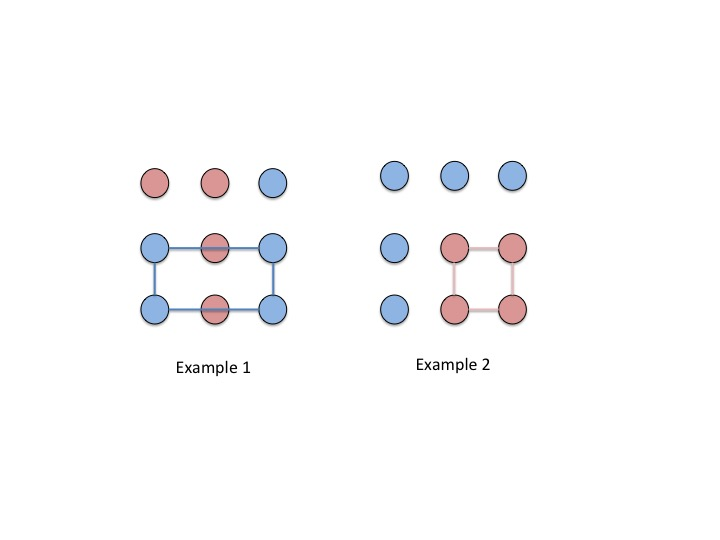
\includegraphics[width=.8\linewidth]{Slide1.jpg}
\end{minipage}

In a 3 x 9 grid there are three dots in each column. Since there are only two colors, red and blue, at least two of the three dots must be the same color (Pigeonhole Principle). Given this restriction there are eight different possible column setups, which can be seen below:

\begin{minipage}{.8\textwidth}
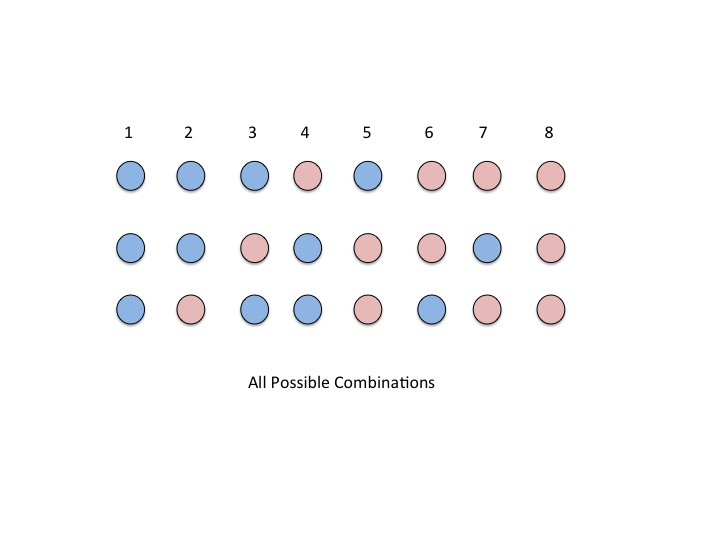
\includegraphics[width=.8\linewidth]{Slide2.jpg}
\end{minipage}

Since there are 9 columns, and 8 possible column formations, one formation must be repeated due to the pigeonhole principle. As shown earlier, this repeated column will form a rectangle with it's duplicate because both columns will have at least two colored points in the same location(either top-bottom, top-middle, or middle-bottom). Therefore, a 3 x 9 grid must contain a rectangle with four points of the same color. 
\end{proof}

\pagebreak
\section*{Problem Six: Properties of Relations: Katie}

\paragraph{i.} The relation $<$ over the set of real numbers is neither an equivalence relation nor a partial order. A common property of equivalence relations and partial orders is that both must be reflexive. This means that every element is related to itself, or formally, that $\forall a \in A.\ aRa$. However, the relation $<$ over the set of real numbers is not reflexive; by the definition of what it means for one quantity to be ``less than" another, it is not the case that $\forall a \in A.\ a<a$. Thus, the relation $<$ is neither an equivalence relation nor a partial order. 

\paragraph{ii.} A relation that is represented by a graph where all nodes have self-edges and there are no edges between distinct nodes is an example of a relation that is both a partial order and an equivalence relation:

\begin{figure}[h]
\centering
  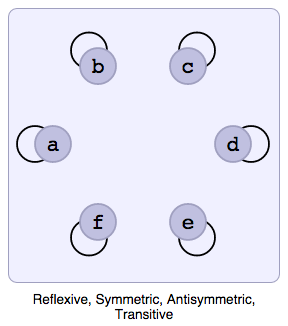
\includegraphics[width=0.45\linewidth]{hw4_6ii.png}
  \caption{A graph where all nodes have self-edges and there are no edges between distinct nodes}
  \label{fig:q6ii}
\end{figure}

In this graph, each node is an element, and an edge from a to b indicates that a is related to b. 

To show that this is a partial order, we show that the relation is reflexive, transitive, and antisymmetric. The relation is reflexive; that is, we drew the graph such that every element is related to itself, or formally, $\forall a \in A.\ aRa$. The relation is transitive; whenever $a$ is related to $b$ and $b$ is related to $c$, we know $a$ is related to $c$, or formally, $\forall a \in A.\ \forall b \in A.\ \forall c \in A.\ (aRb \wedge bRc \rightarrow aRc)$. This is vacuously true, because in the relation we have defined, the antecedent is always false (it is never the case that any element is related to a distinct other object). Finally, the relation is antisymmetric; if $a$ is related to $b$ and $a \neq b$, then $b$ is not related back to $a$, or formally, $\forall a \in A.\ \forall b \in A.\ (a \neq b \wedge aRb \rightarrow \neg(bRa))$. Again, this is vacuously true, because in the relation we have defined, the antecedent is always false (it is never the case that any element is related to a distinct other object).

To show that this is an equivalence relation, we show that the relation is reflexive and transitive (which we have already shown), as well as symmetric. The relation is symmetric; if $a$ is related to $b$, then $b$ is related to $a$, or formally, $\forall a \in A. \forall b \in A.\ (aRb \rightarrow bRa)$. As before, this is vacuously true, because in the relation we have defined, the antecedent is always false (it is never the case that any element is related to a distinct other object).  

The relation we have defined is reflexive, transitive, antisymmetric, and symmetric. Thus, this relation is an example of a relation that is both a partial order and an equivalence relation.

\paragraph{iii.} The relation $=_H$ over P, the set of all people, is an equivalence relation. To show that this is an equivalence relation, we show that $=_H$ is reflexive, transitive, and symmetric. $=_H$ is reflexive; every person is equal in height to themselves, or formally, $\forall p \in P.\ p =_H p$. Next, we show that $=_H$ is transitive; whenever person $p$ is equal in height to person $q$, and person $q$ is equal in height to person $r$, then person $p$ is equal in height to person $r$, or formally, $\forall p \in P.\ \forall q \in P.\ \forall r \in P.\ (p =_H q \wedge q =_H r \rightarrow p =_H r)$. Finally, $=_H$ is symmetric; if person $p$ is equal in height to person $q$, then person $q$ is equal in height to person $p$, or formally, $\forall p \in P. \forall q \in P.\ (p =_H q \rightarrow q =_H p)$. Thus, we have shown that $=_H$ is an equivalence relation.

\paragraph{iv.} The relation $\leq_H$ over P, the set of all people, is not a partial order. To show that this is the case, we show that one of the defining properties of partial orders, antisymmetry, does not hold for the relation $\leq_H$. For a relation to be antisymmetric, it must be the case that:
$$\forall a \in A.\ \forall b \in A.\ (aRb \wedge bRa \rightarrow a=b).$$
Stated in plain English, this says, ``If $a$ is related to $b$ and $b$ is related back to $a$, then $a = b."$ However, we know that this is not the case. There could exist two distinct people, person $p$ and person $q$, where person $p$ is the same height as person $q$. In other words:
$$\exists p \in P.\ \exists q \in P.\ (p \leq_H q \wedge q \leq_H p \wedge p \neq q)$$
This contradicts the property of antisymmetry; we have shown $P \wedge \neg Q$, negating the implication. Because the relation $\leq_H$ is not antisymmetric, we know that it is not a partial order.

\section*{Problem Seven: Meet Semilattices: Marty}

\paragraph{i.} The relation is $<$. If the minimum of (x,y) is always x, then x must be less than y in all cases. 
\paragraph{ii.} The relation is $\subseteq$. For the intersection of x and y to equal x, x must be a subset of y. In a subset relation all elements in x are also present in y, therefore any intersection will equal the entirety of x. 
\paragraph{iii.} 
To prove that relation $\le_S$ is a partial order over D, we must show that it is reflexive, transitive, and antisymmetric.\\
 
\begin{thm} The relation $\le_S$ is reflexive. \end{thm}
\begin{proof} 
A relation is reflexive if  $\forall a \in A. \> aRa.$  In this case we must show that for $\forall x \in D. \ (x \wedge x$ is true). To prove this we know $x \wedge x = x$. $x \wedge x$ can be replaced with x according to the idempotent property. We are then left with $x = x$, therefore $x \wedge x$ is true and the relation $\le_S$ is reflexive.
\end{proof}

\begin{thm} The relation $\le_S$ is transitive. \end{thm}
\begin{proof} A relation is transitive when the following holds: $\forall a \in A .\ \forall b \in A .\ \forall c \in A .\ (aRb \wedge bRc \rightarrow aRc)$. In this case, we want to show that $\forall x \in D .\ \forall y \in D .\ \forall z \in D .\ (x \le_S y \wedge y \le_S z \rightarrow x \le_S z)$. To prove this, we assume that the antecedent is true and show that the consequent must be true as well. We have that both $x \le_S y$ and $y \le_S z$. From the definition of $\le_S$ we know that $x \wedge y = x$ and $y \wedge z = y$. Combining these gives us $x \wedge y \wedge z = x$. 
\begin{align*}
x \wedge y \wedge z &= x \\
x \wedge z &= x
\end{align*}
We have shown that when we assume the antecendent, the consequent is true. This proves that $\le_S$ is transitive.
\end{proof}

\begin{thm} The relation $\le_S$ is antisymmetric. \end{thm}
\begin{proof} A relation is antisymmetric when the following holds: $\forall a \in A .\ \forall b \in A .\ (aRb \wedge bRa \rightarrow a = b)$. In this case, we want to show that $\forall x \in D .\ \forall y \in D .\ (x \le_S y \wedge y \le_S x \rightarrow x = y)$. To prove this, we assume that the antecedent is true and show that the consequent must be true as well. We have that both $x \le_S y$ and $y \le_S x$. From the definition of $\le_S$ we know that $x \wedge y = x$ and $y \wedge x = y$. From the commutative property of the meet semilattice we know that $y \wedge x = x \wedge y = y$. Because $x \wedge y = x$ and $x \wedge y = y$, we know that $x = y$. We have shown that when we assume the antecedent, the consequent must be true. This proves that $\le_S$ is antisymmetric.
\end{proof}

\paragraph{iv.}
\begin{thm} 
For all x,y $\in$D: $x \wedge y \le_S x$
\end{thm} 
\begin{proof}
$x \wedge y \le_S x$ can also be written as $(x \wedge y) \wedge x = x \wedge y$. This equation can then be rearranged using the following properties of $\wedge$:
\begin{align*}
x \wedge (y \wedge x) = x \wedge y \quad Associative\\	
x \wedge (x \wedge y) = x \wedge y \quad Communative\\
(x \wedge x) \wedge y = x \wedge y \quad Associative\\
 x \wedge y = x \wedge y	\quad Idempotent		
\end{align*}
By definition of equality this statement is true, completing the theorem. 
\end{proof} 
\begin{thm} 
For all x,y $\in$D:  $x \wedge y \le_S y$
\end{thm} 
\begin{proof}
$x \wedge y \le_S y$ can also be written as $(x \wedge y) \wedge y = x \wedge y$. This equation can then be rearranged using the following properties of $\wedge$:
\begin{align*}
x \wedge (y \wedge y) = x \wedge y \quad Associative\\	
x \wedge y = x \wedge y \quad Idempotent	
\end{align*}
By definition of equality this statement is true, completing the theorem. 
\end{proof}

\paragraph{v.}
\begin{thm} 
For all x,y,z $\in$D. If $z \le_S x$ and  $z \le_S y$ then $z \le_S x \wedge y$.
\end{thm}
\begin{proof}
If $z \le_S x$ , then:

\begin{align*}
z \wedge x = z.	\quad Equation \>1
\end{align*}

Also if $z \le_S y$, then:
\begin{align*}
z \wedge y = z \quad Equation \> 2
\end{align*}
We will then plug the value for z in equation 2 into equation 1. Which results in $(z \wedge y) \wedge x = z$ This equation can be rearranged using the following properties of $\wedge$:
\begin{align*}
z \wedge (y \wedge x) = z \quad Associative\\ 
z \wedge (x \wedge y) = z \quad Communative
\end{align*}
This final equation can be written as $z \le_S x \wedge y$ using the definition of $\le_S$ . We have reached are desired result, completing the theorem. 
\end{proof}

\section*{Problem Eight: Chains and Antichains: Katie}

\paragraph{i.} The longest chain in the partial order of the $\subseteq$ relation over the set $\wp(\{a, b, c\})$ has a length of 4. An example of such a chain:
$$\emptyset \subseteq \{a\} \subseteq \{a, b\} \subseteq \{a, b, c\}$$

\paragraph{ii.} The largest antichain in the partial order of the $\subseteq$ relation over the set $\wp(\{a, b, c\})$ is a set with a cardinality of 3. An example of such an antichain:
$$\{\{a\}, \{b\}, \{c\}\}$$

\paragraph{iii.} 
\begin{thm} If an arbitrary set A does not contain a chain of length r+1 or greater, then there must be at least s+1 elements of A at the same height, where the height of a is the length of the longest chain whose final element is a. \end{thm}
\begin{proof} Assume A does not contain a chain of length $r+1$ or greater. If this is the case, then the longest possible chain in A is of length $r$. We know that the cardinality of A is $|A| = rs+1$. This means that there are rs+1 elements, which each have heights of at most $r$. 

By the generalized pigeonhole principle, we know that if there are rs+1 elements to put into r possible heights, then there must be some height at which there are at least $\lceil (rs+1)/r \rceil$ elements. We simplify this as follows:
$$\lceil \dfrac{rs+1}{r} \rceil = \lceil \dfrac{r(s+\tfrac{1}{r})}{r} \rceil = \lceil \dfrac{\bcancel{r}(s+\tfrac{1}{r})}{\bcancel{r}} \rceil  = \lceil s+\tfrac{1}{r} \rceil = s+1$$

Thus, we have shown that there must be some height at which there are at least $s+1$ elements of A at that height.
\end{proof}

\paragraph{iv.} 
\begin{thm}X, where X is a set of $s+1$ elements of an arbitrary set A at the same height as one another, must be an antichain.\end{thm}
\begin{proof} First, we begin by stating a new lemma.
\begin{lem} For any arbitrary element $a$ in the longest possible chain ending at $b$, the length of the chain up to $a$ is equal to the height of $a$.
\end{lem}
\begin{proof} By contradiction. Assume that $a$ is an element in the longest possible chain ending at $b$, but the length of the chain up to $a$ is not equal to the height of $a$. Then, by the definition of height, we know that the length of the chain up to $a$ must be less than the height of $a$. If this is the case, then there is another chain ending at $b$ that is even longer, namely the chain where the length of the chain up to $a$ equal to the height of $a$. However, this cannot be true, since we are already working with the longest possible chain ending at $b$. We've reached a contradiction, so our assumption must be false. Thus, if $a$ is an element in the longest possible chain ending at $b$, then the length of the chain up to $a$ must be equal to the height of $a$.
\end{proof}

Now, assume X is a set of $s+1$ elements of A at the same height as one another. Take two arbitrary elements of X, $a$ and $b$. We know that $a$ and $b$ have the same height, $h$. We also know, by \textbf{Lemma 1}, that $a$ cannot be an element of a chain ending at $b$, because this would mean that for the longest possible chain ending at $b$, the chain up to $a$ would have height $h$ (the length of the longest possible chain ending at $a$), which would make the length of the longest possible chain ending at $b$ at least $h+1$. Since we know there are no chains of length greater than $h$ ending at $b$, $a$ could not be an element of a chain ending at $b$. By the definition of a chain, this means that $a$ and $b$ cannot be compared by the partial order relation $\leq_A$.

Thus, we know that for any arbitrary elements $a$ and $b$ in X, $a$ and $b$ cannot be compared by the $\leq_A$ relation. This is the definition of an antichain. Thus, if X is a set of $s+1$ elements of  A at the same height as one another, then X must be an antichain.
\end{proof}

% \section*{Appendix: Referencing Equations}
% \begin{equation} \label{eq:divbyzero}
%   \frac {1} {0}
% \end{equation}

% This references \ref{eq:divbyzero}.

% \section*{Appendix: Figures in Text}
% Below are two different ways of placing figures side by side in text. The first method creates two sub-figures within a single figure. The second method creates two separate figures.

% \begin{figure}
% \centering
% \begin{minipage}{.5\textwidth}
%   \centering
%   \includegraphics[width=.8\linewidth]{hw3_8_1.eps}
%   \captionof{figure}{A figure}
%   \label{fig:q8_test1}
% \end{minipage}%
% \begin{minipage}{.5\textwidth}
%   \centering
%   \includegraphics[width=.8\linewidth]{hw3_8_1.eps}
%   \captionof{figure}{Another figure}
%   \label{fig:q8_test2}
% \end{minipage}
% \end{figure}


% \begin{figure}[h]
%   \centering

%   \begin{subfigure}[b]{0.3\textwidth}
%     \includegraphics[width=\textwidth]{hw3_8_1.eps}
%     \caption{A cycle with length $k+1$}
%     \label{fig:q8_cycle:a}
%   \end{subfigure}% 
%   \qquad
%   \begin{subfigure}[b]{0.3\textwidth}
%     \includegraphics[width=\textwidth]{hw3_8_1.eps}
%     \caption{A cycle with length $k+1$}
%     \label{fig:q8_cycle:b}
%   \end{subfigure}%  

%   \caption{Placeholder}
%   \label{fig:q8}
% \end{figure}

\end{document}
	% line of code telling latex that your document is ending. If you leave this out, you'll get an error

%%% Local Variables:
%%% mode: latex
%%% TeX-master: t
%%% End:
